\section{Implementation and Evaluation}\label{sec:eval}
This section aims to demonstrate that the RVSDG has no inherent
impediment that prevents it from producing competitive code, and that it can
serve as the IR in a compiler's optimization stage.
The goal is not to outperform mature compilers like LLVM or GCC, as it
would require engineering effort far beyond the scope of this article.
We evaluate the RVSDG by generated code performance and size,
compilation time, and representational overhead.


\subsection{Implementation}\label{sec:implementation}

We have implemented \emph{jlm}, a publicly available~\cite{jlm} prototype compiler that uses the
RVSDG for optimizations. Its compilation pipeline is outlined in Figure~\ref{fig:jlmpipeline}. Jlm
takes LLVM IR as input, constructs an RVSDG, transforms and optimizes this RVSDG, and destructs it
again to LLVM IR. The SSA form of the input is destructed before RVSDG construction proceeds with
Inter- and Intra-PT. This additional step is required due to the control flow restructuring phase
of Intra-PT. Destruction discovers control flow by employing SCFR before it constructs SSA form to
output LLVM IR. Jlm supports LLVM IR function, integer, floating point, pointer, array,
structure, and vector types as well as their corresponding operations. Exceptions
and intrinsic functions are currently unsupported. The compiler uses two distinct
states to model side-effects: one for memory accesses and one for
non-terminating loops. We implemented the following optimizations in addition to CNE
and DNE:


\begin{figure*}
	\subfloat[Jlm compilation pipeline.\label{fig:jlmpipeline}] {
		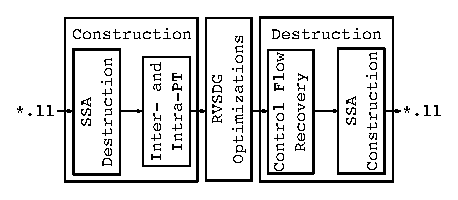
\includegraphics[scale=0.84]{jlmpipeline}
	}
	\hfill
	\subfloat[Evaluation setup.\label{fig:evalsetup}]{
		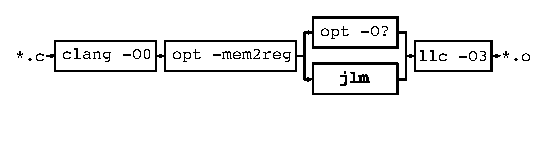
\includegraphics[scale=0.84]{comppipeline}
	}
	\caption{Jlm's compilation pipeline and evaluation setup.}
	\label{fig:pipelines}
\end{figure*}

\begin{itemize}
	\item \textit{Inlining} (ILN): Simple function inlining.

	\item \textit{Invariant Value Redirection} (INV): Redirects invariant values from \thetam and
		\gammanodes.

	\item \textit{Node Push-out} (PSH): Moves all invariant nodes out of \gammam and \thetaregions.

	\item \textit{Node Pull-in} (PLL): Moves all nodes that are only used in one \gammaregion into
		the \gammanode. This ensures their conditional execution, while avoiding code bloat.

	\item \textit{Node Reduction} (RED): Performs simplifications, such as constant folding or
		strength reduction, similarly to LLVM's redundant instruction combinator
		(\texttt{-instcombine}), albeit by far not as many.

	\item \textit{Loop Unrolling} (URL): Unrolls all inner loops by a factor of four. Higher factors
		gave no significant performance improvements in return for the increased code size.

	\item \textit{$\theta-\gamma$ Inversion} (IVT): Inverts \gammam and \thetanodes where both nodes
		have the same predicate origin. This replaces the loop containing a conditional with a
		conditional that has a loop in its then-case.
\end{itemize}

We use the following optimization order: ILN INV RED DNE IVT INV DNE PSH INV DNE URL INV RED CNE
DNE PLL INV DNE.

\subsection{Evaluation Setup}

Figure~\ref{fig:evalsetup} outlines our evaluation setup. We use clang 7.0.1~\cite{clang} to
convert C files to LLVM IR, pre-optimize the IR with LLVM's \texttt{opt}, and then optimize
it either with \texttt{jlm}, or \texttt{opt} using different optimization levels. The optimized
output is converted to an object file with LLVM's \texttt{llc}. The pre-optimization step is
necessary to avoid a re-implementation of LLVM's \texttt{mem2reg} pass, since clang allocates all
values on the stack by default due to LLVM IR only supporting CFGs in SSA form.

We use the polybench 4.2.1 beta benchmark suite~\cite{polybench} to evaluate the RVSDG's
usability and efficacy. This benchmark suite provides structurally small benchmarks, and therefore
reduces the implementation effort for the construction and destruction phases, as well as the
number and complexity of optimizations.

The experiments are performed on an Intel Xeon E5-2695v4 running CentOS 7.4. The
core frequency is pinned to 2.0 GHz to avoid performance variations and thermal throttling effects.
All outputs of the benchmark runs are verified to equal the corresponding outputs of the
executables produced by clang.

\subsection{Performance}

\begin{figure}
	\centering
	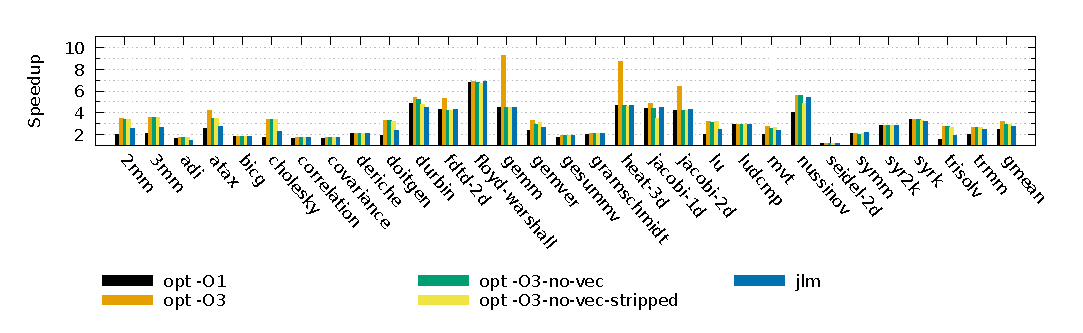
\includegraphics[width=\linewidth]{speedup-LLCO3}
	\caption{Speedup relative to \texttt{O0} at different optimization levels.}
	\label{fig:speedup}
\end{figure}

Figure~\ref{fig:speedup} shows the speedup at five different optimization levels. The \Ozero
optimization level serves as baseline. The \Othreenovec optimization level is the same as
\Othree, but without slp- and loop-vectorization. Optimization level
\Othreenovecstripped is the same as \Othreenovec, but the IR is stripped of named
metadata and attribute groups before invoking \texttt{llc}. Since jlm does not support metadata and
attributes yet, this optimization level permits us to compare the pure optimized IR against jlm
without the optimizer providing hints to \texttt{llc}. We omit optimization level \Otwo as
it was very similar to \Othree. The gmean column in Figure~\ref{fig:speedup} shows the
geometric mean of all benchmarks.

The results show that the executables produced by jlm (gmean 2.70) are faster than \Oone
(gmean 2.49), but slower than \Othree (gmean 3.22), \Othreenovec (gmean 2.95), and
\Othreenovecstripped (gmean 2.91). Optimization level \Othree attempts to vectorize
twenty
benchmarks, but only produces measurable results for eight of them: atax, durbin,
fdtd-2d, gemm, gemver, heat-3d, jacobi-1d, and jacobi-2d. Jlm would require a vectorizer to
achieve such speedups.

Disabling vectorization with \Othreenovec and \Othreenovecstripped shows that jlm
achieves similar speedups for fdtd-2d, gemm, heat-3d, javobi-1d, and jacobi-2d. The metadata
transferred between the optimizer and \texttt{llc} only makes a significant difference for durbin,
floyd-warshall, gesummv, jacobi-1d, and nussinov. In the case of gesummv and jacobi-1d, performance
drops below jlm.
Jlm is outperformed by optimization level \Oone at four benchmarks: adi, durbin, seidel-2d, and
syrk. We inspected the output files and found the following causes:

\begin{itemize}
	\item \textit{adi}: Jlm fails to eliminate load instructions from the two innermost loops. These
		loads have loop-carried dependencies with a distance of one to store instructions in the same
		loop, and can be eliminated by propagating the stored value to the users of the load's
		output. The corresponding LLVM pass is loop load elimination
		(\texttt{-loop-load-elim}). Jlm performance equals \Oone
        if this transformation is performed by hand.

	\item \textit{durbin}: Jlm fails to transform a loop that copies values between arrays to a
		\texttt{memcpy} intrinsic. This impedes LLVM's code generator to produce better code. The LLVM
		pass responsible for this transformation is the loop-idiom pass (\texttt{-loop-idiom}). If the
		loop is replaced with a call to \texttt{memcpy}, then jlm is better than \Oone.



	\item \textit{seidel-2d}: Similarly to adi, jlm fails to eliminate load instructions from
		the innermost loop. If the load elimination is performed by hand, then jlm achieves the
		same performance as \Oone.

	\item \textit{syrk}: Jlm fails to satisfactorily apply CNE due to an overly strict
		sequentialization of load and store instructions. Loads from the same address are not detected
		as congruent due to different state edge origins. An alias analysis pass would resolve this
		problem.
\end{itemize}

Figure~\ref{fig:speedup} shows that it is feasible to produce competitive code using the RVSDG,
but also that more optimizations and analyses are required in order to
reliably do so. Performance differences are not caused by inherent RVSDG characteristics,
but can be attributed to missing analyses, optimizations, and heuristics for their
application.
The above results and Table~\ref{tab:llvm-opts} indicate that an alias analysis
pass is particluarly required.

\subsection{Code Size}

\begin{figure}
	\centering
	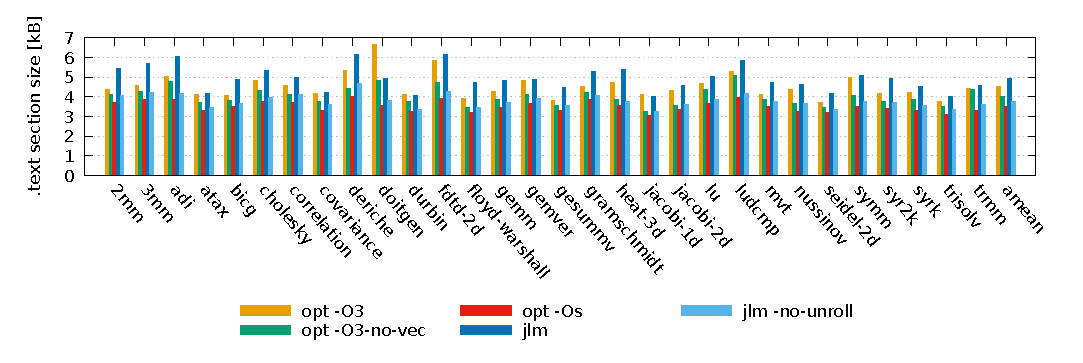
\includegraphics[width=\linewidth]{codesize}
	\caption{Code size at different optimization levels.}
	\label{fig:codesize}
\end{figure}

Figure~\ref{fig:codesize} shows the code size for \Othree, \Othreenovec, \Os,
and for jlm with and without loop unrolling. The amean column shows the arithmetic mean of all
benchmarks.
Optimization level \Othree produces on average text sections that are 11\% bigger than
\Othreenovec. Vectorization often requires loop transformations to make
loops amenable to the vectorizer, and the insertion of pre- and post-loop code. This affects code
size negatively, but can result in better performance.
The results also show that \Os produces smaller text sections than
\Othreenovec. This is due to more conservative optimization heuristics and the omission of
optimizations, \eg, aggressive instruction combination (\texttt{-aggressive-instcombine}) or
the promotion of by-reference arguments to scalars (\texttt{-argpromotion}).

Jlm produces ca. 39\% bigger text sections compared to \Os. The results
without loop unrolling show that this can be attributed to the naive heuristic used. Jlm does not
take code size into account and unrolls every inner loop unconditionally
four times, leading to excessive code expansion. Avoiding unrolling completely results in text
sections that are on average between \Othreenovec and \Os. This indicates that the
excessive code size is due to naive heuristics and shortcomings in the implementation, but not to
inherent characteristics of the RVSDG.

\subsection{Compilation Overhead}

\begin{figure*}
	\subfloat[Representational overhead.\label{fig:repoverhead}] {
		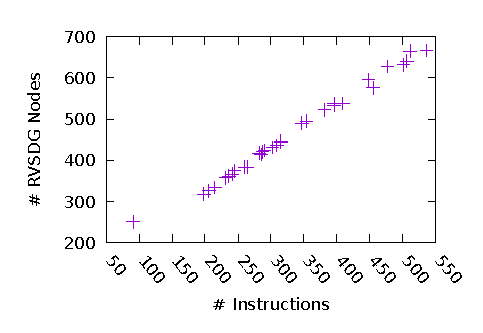
\includegraphics[scale=0.89]{iroverhead}
	}
	\hfill
	\subfloat[Compilation times.\label{fig:timeoverhead}] {
		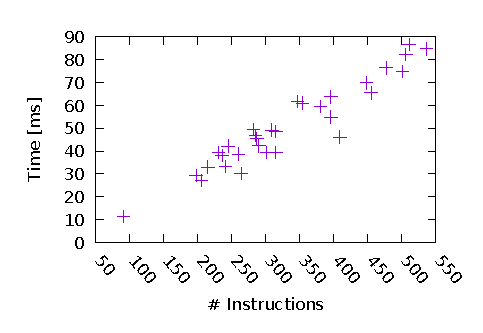
\includegraphics[scale=0.89]{jlmtime}
	}
	\caption{Compilation overhead of jlm.}
	\label{fig:overhead}
\end{figure*}

Figure~\ref{fig:overhead} shows overhead in terms of IR size and time, with
Figure \ref{fig:repoverhead} relating LLVM instruction count to number of
RVSDG nodes, and Figure \ref{fig:timeoverhead} relating it to time spent on
RVSDG translation and optimizations.

Figure~\ref{fig:repoverhead} shows a clear linear relationship for all cases, confirming the
observations by Bahmann~\etal~\cite{Bahmann15} that the RVSDG is feasible in terms of space
requirements. Figure~\ref{fig:timeoverhead} also indicates a linear dependency, but with larger
variations for similar input sizes. We attribute this variation to the fact that construction,
optimizations, and destruction are also compounded by input structure. Structural
differences in the inter-procedure and control flow graphs lead to runtime variations in RVSDG
construction and destruction, as well as different runtimes for optimizations. For example, the
presence of loops in a translation unit determines whether loop unrolling is performed, while their
absence incurs no runtime overhead.
Figure~\ref{fig:overhead} shows that the RVSDG is feasible as an IR for optimizing
compilers in terms of compilation overhead.

\subsection{Comparison to LLVM}\label{sec:llvm-comparison}

LLVM 7.0.1 invokes 85 different analyses and optimization passes at optimization level \texttt{O3}.
Many of these passes are repeatedly invoked, resulting in a total of 266 invocations.
Section~\ref{sec:rep-invariants} already highlighted that 57, or 21\%, of these invocations are
from six helper passes that only establish invariants and detect structures necessary for
optimizations. Table~\ref{tab:llvm-opts} in Section~\ref{sec:rep-invariants} also shows that
LLVM necessitates SSA restoration in
fourteen optimization passes.
Because LLVM's CFG representation does not maintain necessary invariants and structures,
it requires (re-)computation of their information, which leads to a high number of
helper pass invocations.
This can
be observed in LLVM's optimization pipeline for loop optimizations:
... \emph{-loops -loop-simplify -lcssa-verification -lcssa} ... -loop-rotate -licm
-loop-unswitch \emph{-loop-simplify -lcsse-verification -lcssa} .... -loop-idiom -loop-deletion
-loop-unroll ... \emph{-loops -loop-simplify -lcssa-verification -lcssa} ... -loop-rotate
-loop-accesses ... . Depending on an optimization's position in the pipeline, several
helper passes must be executed before an optimization can be invoked. This is necessary to ensure
that the required information for an optimization is present, and up to date after 
invocation of other optimizations, \eg, jump threading (\texttt{-jump-threading}) or
CFG simplification (\texttt{-simplifycfg}). Thus, each added loop optimization
can necessitate several more helper passes in the optimization pipeline. A
similar pattern is seen with (basic) alias analysis (\texttt{-basicaa} and \texttt{-aa}),
which are invoked 37 times in total.

In contrast, the RVSDG establishes the necessary invariants and structures during construction,
and maintains them throughout compilation. The result is that jlm requires none of the
aforementioned helper passes and SSA restoration, \eg,
loop unrolling (URL) can be readily performed without the need to detect loops, their entry,
and exits. The cost is a more elaborate construction, which requires the
detection of the necessary information, and destruction, which requires the recovery
of control flow. However, RVSDG construction and destruction only need to be performed once
and, as demonstrated in Section~\ref{fig:overhead} and in Bahman~\etal~\cite{Bahmann15}, are
practically feasible.


